%%%%%%%%%%%%%%%%%%%%%%%%%%%%%%%%%%%%%%%%%%%%%%%%%
% Introduction
%%%%%%%%%%%%%%%%%%%%%%%%%%%%%%%%%%%%%%%%%%%%%%%%%
\subsection{Introduction}
\label{fpga:Introduction}
In the two decades since \glspl{FPGA} were introduced, they have radically
changed the way digital logic is designed and deployed \cite{Hauck:2007}.
\glspl{FPGA} are revolutionary devices that offer a compromise between the
flexibility and ease of microprocessor-based software designs; and the
performance and efficiency of \gls{ASIC}-based hardware design. Unlike an
\gls{ASIC}, computations are programmed into the \gls{FPGA} device, instead of
being permanently constructed during the manufacturing process. This means that
an \gls{FPGA} device can be programmed and reprogrammed ny times, allowing for
a significant level of flexibility whilst enabling a much faster and efficient
implementation than a software equivalent.

These benefits, however, do not come without a cost. Designing an
\gls{FPGA}-based system is a more complicated process than the development of a
software process. In order to effectively utilise hardware resources, the
designer of an \gls{FPGA}-based system must consider the hardware resources that
are provided by the \gls{FPGA} device, and must remain flexible during the
design process so as to utilise as many of the hardware resources that are
available whilst ensuring that the highest level of performance is obtained.
These considerations are seldom necessary in a pure-software approach, as tools
such as compilers and assemblers abstract the hardware implementation details
away from the developers in order to provide cross-system and, often,
cross-architecture compatability.

Compared to an \gls{ASIC} design, which may take many months or years to design
and have a multimillion-dollar price tag, an \gls{FPGA} design might only take
days to create and cost tens to hundreds of dollars \cite{Hauck:2007}.

\begin{figure}
    \centering
    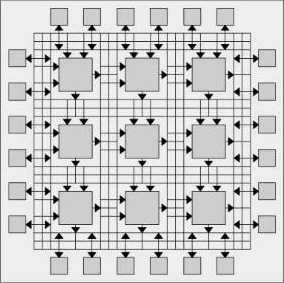
\includegraphics[width=0.5\textwidth]{fpga/abstract-view}
    \caption[An abstract view of an \gls{FPGA}.]
        {An abstract view of an \gls{FPGA} \cite{Hauck:2007}.}
    \label{fig:fpga:abstract}
\end{figure}

\autoref{fig:fpga:abstract} shows an abstract view of an \gls{FPGA}, which
consists of an \emph{array} of logic blocks (\emph{gates}) connected in a
general routing structure. THe logic blocks contains processing elements for
impleenting combinatorial logic, as well as flip-flops for implementing
sequential logic. The logic and routing elments of an \gls{FPGA} are controlled
by programming points, which may be based on anitfuse, Flash  or \gls{SRAM}
technology. With the corresponding memory bits programmed, by way of a
configuration file or a bitstream, an \gls{FPGA} can be made to implement the
user's desired function. For this reason, glspl{FPGAs} are referred to as
\emph{field progammable} devices, as opposed to \emph{mask programmable}
devices, which have their  functionality fixed by masks during fabrication.

The design of an \gls{FPGA} program typically begins with an algorithm expressed
in a \gls{HDL} such as Verilog or \gls{VHDL}. An \gls{FPGA} design goes through
several development phases \cite{Hauck:2007}:
\begin{description}
    \item[Logic synthesis] Converts high level logic constructs and behavioural
        code into gates.
    \item[Technology mapping] Separate the gates into groupings that best match
        the \gls{FPGA}'s logic resources.
    \item[Placement] Assigns the logic groupings to specific logic blocks.
    \item[Routing] Determines the interconnect resources that will carry the
        user's signals.
    \item[Bitstream generation] Creates a binary file that sets all of the
        \gls{FPGA}'s programming points to configure the logic blocks and
        routing resources appropriately.
\end{description}

%%%%%%%%%%%%%%%%%%%%%%%%%%%%%%%%%%%%%%%%%%%%%%%%%
% Device architecture
%%%%%%%%%%%%%%%%%%%%%%%%%%%%%%%%%%%%%%%%%%%%%%%%%
\subsection{Device architecture}
\label{fpga:deviceArchitecture}
% TODO

% Logic elements
\paragraph{Logic elements}
\label{fpga:deviceArchitecture:logicElements}
% TODO

% The array and interconnect
\paragraph{The array and interconnect}
\label{fpga:deviceArchitecture:arrayAndInterconnect}
% TODO

% Configuration
\subsubsection{Configuration}
\label{fpga:deviceArchitecture:conf}
% TODO

\paragraph{\gls{SRAM}}
\label{fpga:deviceArchitecture:sram}
% TODO

\paragraph{Flash memory}
\label{fpga:deviceArchitecture:flash}
% TODO

\paragraph{Antifuse}
\label{fpga:deviceArchitecture:antifuse}
% TODO

\paragraph{Configuration}
\label{fpga:deviceArchitecture:conf}
% TODO
